%% PCDG — WWW 2027 submission (Research Track)
%% Double-blind, review mode. Compile with:  latexmk -pdf main.tex
\documentclass[sigconf,anonymous,review]{acmart}

% ---- review / draft conveniences (remove `review` and set copyright for camera-ready) ----
\settopmatter{printacmref=false}          % suppress ACM reference block during review
\setcopyright{none}                        % anonymous review; set properly for camera-ready
\acmConference[WWW '27]{Proceedings of the ACM Web Conference 2027}{May 10--14, 2027}{Dublin, Ireland}
\acmDOI{}
\acmISBN{}
\renewcommand{\footnotetextcopyrightpermission}[1]{}

\usepackage{booktabs}
\usepackage{amsmath}
\usepackage{amssymb}
\usepackage{graphicx}
\usepackage{xcolor}
\usepackage{enumitem}
\usepackage{algorithm}
\usepackage{algpseudocode}

% draft-only helper; make it a no-op before submission
\newcommand{\todo}[1]{\textcolor{red}{\small[TODO: #1]}}
% shared macros
\newcommand{\pcdg}{\textsc{PCDG}\xspace}
\newcommand{\pcdgp}{\textsc{PCDG-P}\xspace}
\newcommand{\pcdgpd}{\textsc{PCDG-PD}\xspace}
\usepackage{xspace}
\newcommand{\Mmat}{\mathbf{M}}
\newcommand{\dkl}{D_{\mathrm{KL}}}
\newcommand{\relu}{\mathrm{ReLU}}

\begin{document}

\title{Training-Free Partial-Order Control for Discrete-Diffusion POI Check-in Generation}

% ---- Author block ----
% Order and names are LOCKED at the 2026-10-18 abstract registration.
% FILL BEFORE CAMERA-READY: both e-mail addresses below are UNVERIFIED placeholders, and
% neither ORCID has been supplied. Replace with the real values; do not guess an ORCID.
% NOTE: the `anonymous` class option blanks this block in the review PDF, so these names
% are not disclosed by the submitted file. They are still needed in the registration form.
\author{Zhiyi Li}
\email{TODO-confirm@hit.edu.cn}            % placeholder, not verified
\affiliation{%
  \institution{School of Computer Science and Technology, Harbin Institute of Technology, Shenzhen}
  \city{Shenzhen}
  \country{China}
}

\author{Kaiqi Zhao}
\authornote{Corresponding author.}
\email{TODO-confirm@hit.edu.cn}            % placeholder, not verified
\affiliation{%
  \institution{School of Computer Science and Technology, Harbin Institute of Technology, Shenzhen}
  \city{Shenzhen}
  \country{China}
}

\renewcommand{\shortauthors}{Li and Zhao}

\begin{abstract}
Location-based social networks (LBSNs) are a core source of web-scale human-mobility
data, yet sharing raw check-in traces is privacy-sensitive, motivating realistic
synthetic generation. Beyond statistical realism, many downstream web applications need
control over the \emph{semantic order} of activities---e.g., leisure before dining---a
sample-level, cross-position requirement that single-step conditioning cannot express.
Enforcing such constraints is commonly assumed to cost distributional fidelity; we show
this trade-off is largely \emph{separable}. We present \pcdg, a \emph{training-free}
control stack for a frozen conditional joint temporal\,+\,category/POI
discrete-diffusion generator. \pcdg compiles category partial-order constraints into
differentiable energies, projects the category-position logits through a KL-preserving
augmented-Lagrangian optimization in the late reverse steps, eliminates residual
category--POI inconsistency via a category-consistent decoder, and restores spatial
realism through a distribution-aware same-category geometry refinement that leaves every
constraint metric unchanged \emph{by construction}. Across two cities under an
out-of-distribution split and three sampling seeds, \pcdg cuts the strict
ordering-violation rate from $92.89\%$ to $4.04\%$ on Istanbul and from $89.45\%$ to
$11.28\%$ on New York, raising pairwise ordering coverage by $6.5\times$ and
$4.2\times$, while \emph{improving} all six fidelity divergences over the unconstrained
backbone on Istanbul and four of six on New York. On Istanbul it surpasses a
\emph{fully retrained} partial-order conditional model on all five constraint metrics and
five of six fidelity divergences, without retraining anything. Stage-wise ablations
localize where fidelity is lost and recovered across the three-stage stack.
\end{abstract}

% ---- CCS ----
% NOT needed for the 10-18 abstract registration. These two concepts are the ones
% inherited from the thesis draft; regenerate the whole block from the official ACM CCS
% tool (https://dl.acm.org/ccs) before the full-paper deadline rather than hand-editing
% concept_ids, which must match ACM's taxonomy exactly.
\begin{CCSXML}
<ccs2012>
   <concept>
       <concept_id>10010147.10010257.10010258.10010259</concept_id>
       <concept_desc>Computing methodologies~Machine learning</concept_desc>
       <concept_significance>500</concept_significance>
   </concept>
   <concept>
       <concept_id>10002951.10003227</concept_id>
       <concept_desc>Information systems~Information systems applications</concept_desc>
       <concept_significance>300</concept_significance>
   </concept>
</ccs2012>
\end{CCSXML}
\ccsdesc[500]{Computing methodologies~Machine learning}
\ccsdesc[300]{Information systems~Information systems applications}

\keywords{synthetic human mobility, discrete diffusion, partial-order constraints,
training-free constrained sampling, POI check-in sequences}

\maketitle

\section{Introduction}
\label{sec:intro}

Location-based social networks (LBSNs) and location-aware web services generate
vast streams of \emph{check-in} data: time-stamped visits to points of interest
(POIs), each carrying an activity semantics such as dining, leisure, or shopping.
These web-scale traces underpin POI recommendation, urban analytics, and mobility
simulation~\cite{feng2018deepmove,luo2021stan,yang2022getnext}. Yet releasing raw
traces is privacy-sensitive, and long-tail scenarios are scarce, which has made
the generation of realistic \emph{synthetic} mobility an active research
direction~\cite{feng2020simulate,yuan2022activity,long2023synthetic,deng2025marionette}.

Most prior generators optimize statistical realism alone. Many web applications,
however, require \emph{control over activity semantics}---in particular, over the
\emph{order} in which categories of activities occur. A scenario designer may need
sequences in which leisure precedes dining, or sightseeing precedes shopping, in
order to study specific behavioral patterns, stress-test a recommender, or
augment data for a target scenario. Such a requirement is a \emph{sample-level
partial order} over categories: it couples multiple, possibly non-adjacent
positions of a sequence and therefore cannot be expressed by reweighting any
single token, nor by next-location prediction, which outputs one step at a time
rather than a complete constrained sequence.

Enforcing such constraints is surprisingly hard for modern generators. Generating
freely and then \emph{reordering} the output satisfies the constraint but distorts
the jointly learned distribution over time, category, and space. Classifier-free
or classifier-based guidance can bias generation toward a condition, but a
condition embedding does not \emph{guarantee} a global ordering, and retraining a
conditional model for every constraint family is expensive and city-specific.
Recent work on controllable trajectory generation enforces \emph{geometric}
constraints such as road topology~\cite{zhu2024controltraj}, and generic
constrained discrete diffusion enforces sequence-level logical
constraints~\cite{cardei2025cdd}; neither has been specialized to the activity-%
category precedence that arises in POI check-in sequences, nor to the joint
temporal\,+\,category\,+\,POI setting.

We introduce \pcdg, a \emph{training-free} control stack that enforces sample-level
category precedence directly inside the reverse diffusion of a frozen conditional
generator, and that---crucially---does so without paying the fidelity penalty such
control is usually assumed to require. \pcdg has three sampling-time stages. First, it
compiles a partial-order matrix into differentiable order-violation and existence
energies and, during the late reverse steps, projects \emph{only the category-position
logits} via a KL-preserving augmented-Lagrangian optimization. Second, a
category-consistent POI decoder resolves the residual mismatch between a sampled
category and the POI actually emitted at that position. Third, a distribution-aware
same-category geometry refinement re-selects each POI among candidates of the
\emph{same} realized category so as to match population-level travel-length and
visitation statistics; because it never touches category tokens, times, lengths or
order, it leaves every constraint metric unchanged by construction. Because all three
stages read and rewrite only the per-step sampling distribution and the realized POI
assignment of a frozen model, \pcdg adds no parameters, needs no retraining, and can be
attached to an existing, already-deployed generator.

Our analysis traces the fidelity cost of constrained sampling to two separable
sources---an over-weighted constraint penalty inside the projection, and a
POI/coordinate selection that is blind to the population spatial distribution---and
shows that correcting them recovers, and on one city surpasses, the unconstrained
generator's fidelity while retaining almost all of the constraint gain.

\paragraph{Relevance to the Web.}
This work studies the Web as a socio-economic system and a responsible-data
problem. LBSN check-in logs are a native web data source that powers POI
recommendation and urban web services, but releasing raw traces risks user
privacy. Generating controllable, constraint-satisfying synthetic mobility lets
practitioners share and augment web-behavior data while honoring
application-specified activity semantics, directly serving privacy-conscious web
data sharing and downstream recommendation. The method also contributes a reusable
recipe---training-free, sampling-time constraint projection on a frozen
generator---for controllable generation of other structured web content.

\paragraph{Contributions.}
\begin{itemize}[leftmargin=1.2em,itemsep=2pt,topsep=2pt]
  \item We formalize \emph{category partial-order constrained POI check-in
  generation}---a sample-level, cross-position precedence requirement with an
  anti-degeneracy existence condition---and express it as differentiable energies
  compatible with discrete-diffusion sampling (\S\ref{sec:problem},
  \S\ref{sec:method:energy}).
  \item We propose \pcdg, a three-stage \emph{training-free} sampling-time control stack
  on a \emph{frozen} joint temporal\,+\,category\,+\,POI diffusion generator: a
  KL-preserving augmented-Lagrangian projection of the category-position logits,
  category-consistent POI decoding, and a distribution-aware same-category geometry
  refinement that is constraint-neutral by construction (\S\ref{sec:method}).
  \item We show that the fidelity--constraint trade-off reported for constrained
  sampling is \emph{separable} rather than intrinsic: it decomposes into an
  over-weighted constraint penalty and a distribution-blind POI/coordinate selection.
  Correcting both recovers the unconstrained generator's fidelity on every measured
  divergence on one city, and the configuration that wins uses \emph{no}
  category-side distribution term, localizing the loss to the spatial side
  (\S\ref{sec:exp:tradeoff}).
  \item We conduct a two-city, out-of-distribution, multi-seed study with a projection
  ablation and a stage-wise ablation of the full stack, showing that \pcdg attains the
  strongest constraint satisfaction among energy-guidance, post-hoc, and even
  \emph{fully retrained} conditional baselines while matching or beating them on
  fidelity, and we report the two New York statistics that remain above the
  unconstrained backbone (\S\ref{sec:experiments}).
\end{itemize}

\section{Related Work}
\label{sec:related}

\paragraph{Human mobility and POI modeling.}
Classical studies established that human movement is highly regular yet only
boundedly predictable~\cite{gonzalez2008mobility,song2010predictability}. A large
body of work predicts the \emph{next} location from history using attentional,
spatio-temporal, and graph-enhanced
models~\cite{feng2018deepmove,luo2021stan,yang2022getnext}, and diffusion models
have recently been applied to next-POI and sequential
recommendation~\cite{long2024cloudedge,wang2024dsdrec,chen2025sequentialdiffusion,qin2023diffpoi,wang2025gnprsid}.
These prediction and ranking objectives differ from generating complete
time-stamped visits under sample-level activity-order requirements.

\paragraph{Synthetic trajectory and mobility generation.}
Data-driven generation spans GAN/Seq2Seq
models~\cite{cao2021trajgen,jiang2023tstrajgen,xiong2024trajsgan,lin2023mbpgail},
point-process and neural-ODE
generators~\cite{yuan2022activity,long2023synthetic}, imitation- and
privacy-oriented
approaches~\cite{feng2020simulate,wang2023pategail,sun2023sprt,rao2023cats,hu2024retrasyn,netzler2024privacy},
and, increasingly, diffusion
models~\cite{zhu2023difftraj,yuan2023stdpp,gong2025stcdm,chen2024trajgdm,wei2024diffrntraj,rao2025seed,long2026population}
and Transformer/LLM-based
generators~\cite{zhang2024mobglm,hsu2024trajgpt,li2025geollama,haydari2026mobilitygpt}.
Marionette supports fine-grained generation using global and partial mobility
contexts~\cite{deng2025marionette}; we use its generator as a frozen backbone.
Related benchmarks examine imitative generation quality~\cite{deng2025mirage}.
Our target is an explicit relation between activity categories, together with
the distributional effects of enforcing it on generated POI identities.

\paragraph{Discrete diffusion.}
Discrete diffusion extends denoising diffusion~\cite{ho2020ddpm} to categorical
data via structured transition matrices~\cite{austin2021d3pm}, concrete score
matching~\cite{meng2022concrete}, score-entropy~\cite{lou2024sedd}, and masked
formulations~\cite{sahoo2024mdlm}. Discrete classifier-free and classifier-based
guidance steer generation toward conditions~\cite{schiff2025guidance}.
Our EnergyGuide baseline instead takes a gradient of the local order/existence
energy; it does not reproduce that work's classifier-likelihood construction.
\pcdg intervenes in the frozen backbone at sampling time.

\paragraph{Sampling-time constraint projection.}
CDD integrates differentiable constraints into discrete-diffusion sampling
through KL anchoring and augmented-Lagrangian optimization without
retraining~\cite{cardei2025cdd}. We adapt that projection mechanism to order and
existence energies on category positions. The KL anchor penalizes token-level
drift from the denoiser; matching aggregate travel-distance and visitation
statistics to training references is a separate objective in our stack.
We evaluate those terms through projection and stage-wise comparisons rather
than treating the KL anchor as a distributional-fidelity guarantee.

\paragraph{Decoding support and spatial refinement.}
Grammar-constrained decoding restricts language-model outputs to permitted
formal structures~\cite{geng2023grammar}; Control-DAG uses weighted finite-state
automata for lexical, vocabulary, and length control in non-autoregressive
generation~\cite{chen2024controldag}. Our decoder instead couples category tokens
to admissible catalog POIs. Its final-category fallback prevents a universal
consistency guarantee. Geographic control is complementary: ControlTraj uses
road topology and trip attributes to condition trajectory
generation~\cite{zhu2024controltraj}. This differs from preserving an activity
sequence while changing its locations. Our terminal refinement reselects POIs
within their realized categories; the stage-wise evaluation measures how much
spatial fidelity this restriction permits us to recover, and which errors remain.

\section{Problem Definition}
\label{sec:problem}

\begin{definition}[POI check-in sequence]
A POI check-in sequence of length $n$ is
$s=(t_{1:n},k_{1:n},l_{1:n})$, where $t_{1:n}$ are arrival times,
$k_i \in \mathcal{C}=\{1,\dots,C\}$ are activity categories; $\mathcal{C}$ is
the category set and $C=|\mathcal{C}|$ its size; and
$l_i \in \mathcal{L}$ are points of interest. Each POI $l$ has fixed
coordinates $\mathrm{gps}(l)$ and a catalog category $\mathrm{cat}(l)$.
\end{definition}

\begin{definition}[Context]
The context supplied with a sequence is a tuple
$\mathbf{c}=(\mathbf{c}^{(1)},\dots,\mathbf{c}^{(R)})$, where each
$\mathbf{c}^{(r)}$ is one condition channel represented over fixed within-day
bins. A channel may encode a day-level calendar or behavioral label that
persists across the sequence, or a partial condition that varies over the day.
The context conditions generation of the complete sequence; generated event
times $t_{1:n}$ remain separate temporal variables.
\end{definition}

The backbone has six condition channels encoded over $24$ daily windows. The
Istanbul setup described by Marionette uses day of week, Ramadan, public
holidays, and hour of day; the first three are global and the last is partial.
This study's New York preprocessing encodes day of week, a U.S. federal-holiday
flag, and season; its other three channels are constant-coded. The window axis
indexes context, not event times $t_{1:n}$. Context does not assign POI
identities or specify required categories or their partial order.
The generator's category token $k_i$ and the emitted POI's catalog category
$\mathrm{cat}(l_i)$ are separate outputs, and the latter determines the
realized activity.

\begin{definition}[Category partial-order matrix]
A category partial-order matrix is a binary matrix
$\Mmat\in\{0,1\}^{C\times C}$, where $\Mmat[a,b]=1$ denotes the strict
precedence requirement that category $a$ precede category $b$, and
$\Mmat[a,b]=0$ denotes no such requirement.
\end{definition}

Both user-specified partial-order constraints and a reference check-in
sequence induce a matrix of this form. For a sequence $s$, let
$I_s(a)=\{i:\mathrm{cat}(l_i)=a\}$ be the positions whose realized POI
category is $a$. Its induced matrix is
\begin{equation}
  \widehat{\Mmat}(s)[a,b]=
  \begin{cases}
    1, & I_s(a),I_s(b)\neq\varnothing\text{ and }\max I_s(a)<\min I_s(b),\\
    0, & \text{otherwise}.
  \end{cases}
  \label{eq:induced-po-matrix}
\end{equation}
For user-specified relations, $\Mmat[a,b]=1$ whenever $a$ is required to
precede $b$; for a reference sequence $s_{\mathrm{ref}}$, we set
$\Mmat=\widehat{\Mmat}(s_{\mathrm{ref}})$. A missing category or an inversion
sets the corresponding induced entry to zero.

\begin{definition}[Partial-order-constrained POI generation]
Given a frozen conditional generator $p_\theta(s\mid\mathbf{c})$ and a target
matrix $\Mmat$, sampling-time control produces
\begin{equation}
  \hat{s}\sim p_{\mathrm{PCDG}}(s\mid\mathbf{c},\Mmat),
  \qquad
  \Mmat[a,b]\leq\widehat{\Mmat}(\hat{s})[a,b]
  \quad\forall a,b,
  \label{eq:task}
\end{equation}
or, equivalently,
\[
  \Mmat\odot\bigl(\mathbf{1}_{C\times C}-\widehat{\Mmat}(\hat{s})\bigr)=0.
\]
\end{definition}

The condition in~\eqref{eq:task} checks only relations required by $\Mmat$;
additional valid relations are allowed. A relation fails if either category is
absent or their order is inverted. Since $\widehat{\Mmat}$ uses
$\mathrm{cat}(l_i)$, satisfaction is measured on realized POI categories.
Unlike next-location prediction~\cite{feng2018deepmove,luo2021stan,yang2022getnext},
the task generates a complete time-stamped, categorized, geolocated sequence
under constraints coupling multiple, potentially non-adjacent positions.

We evaluate distributional fidelity and satisfaction of the required category
orders. The former compares generated and reference mobility statistics; the
latter checks whether required categories appear and occur in the requested
order. Section~\ref{sec:exp:metrics} and Appendix~\ref{app:metrics} define the
statistics and their aggregation rules. Together they distinguish correct
ordering from apparent satisfaction caused by omitting required activities.

\section{Method}
\label{sec:method}

\pcdg controls a frozen generator through sampling-time logit projection,
category-consistent POI decoding, and terminal same-category refinement
(Figure~\ref{fig:framework}). The weights $\rho,\lambda,\beta$ enter their objectives.
\begin{figure*}[t]
  \centering
  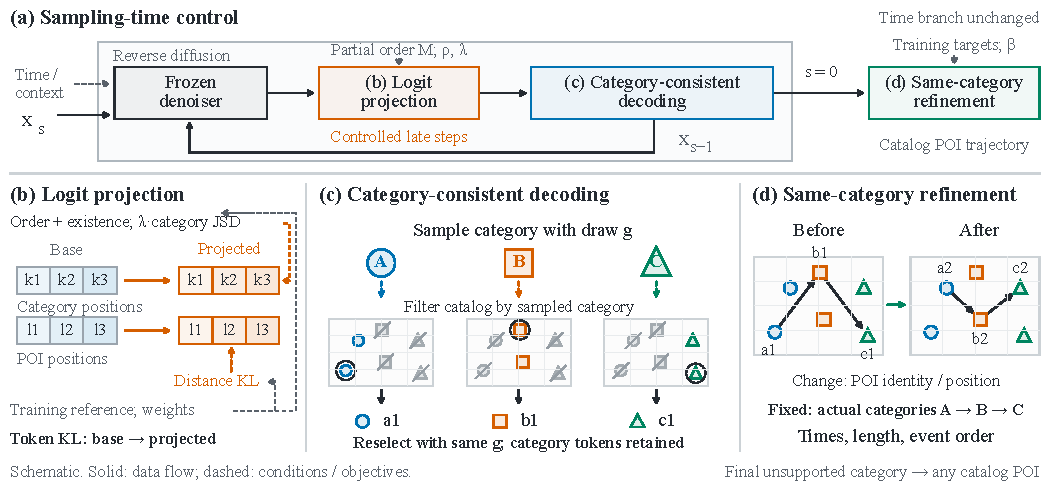
\includegraphics[width=\textwidth]{figures/framework.pdf}
  \caption{\pcdg (schematic). (a) Frozen reverse loop and terminal refinement.
  (b) Category order/existence energies and POI distance KL, anchored by base-to-projected token KL.
  (c) Category-filtered POI reselection reuses Gumbel noise.
  (d) Same-frame refinement preserves actual categories, times, length, and order.
  Dashed edges carry conditions/objectives.
  Intermediate steps allow POI masks and leave unresolved categories unfiltered.
  Unsupported final categories allow any catalog POI, permitting nonzero mismatch.}
  \Description{Four panels trace sampling-time category control. Panel a places a
  frozen denoiser, late-step logit projection, and category-consistent decoding
  inside a reverse-diffusion loop, followed by terminal same-category refinement.
  Panel b separates category and POI logit positions and their objectives.
  Panel c uses blue circles A, orange squares B, and green triangles C for three
  events. Each sampled category filters a common six-POI catalog; incompatible
  candidates are gray and crossed out. Shared-noise reselection yields a1, b1, c1.
  Panel d uses the same coordinates to replace these with a2, b2, c2 while retaining
  actual categories, times, length, and event order. A note marks the final
  unsupported-category fallback to any catalog POI.}
  \label{fig:framework}
\end{figure*}

\subsection{Backbone: conditional joint discrete diffusion}
\label{sec:method:backbone}
The current implementation uses a frozen generator whose discrete branch follows the Marionette-style diffusion point process for arrival times and conditional
discrete diffusion for categories and POIs~\cite{deng2025marionette}. Its discrete
branch represents a sequence as
$\mathbf{x}=[\textsc{start},\,k_{1:n},\,\textsc{sep},\,l_{1:n},\,\textsc{end}]$,
with a \emph{category mask} and a \emph{POI mask} identifying the two segments.
Categories and POIs use separate absorbing-state transition
matrices~\cite{austin2021d3pm}; a Transformer denoiser with an
$\mathbf{x}_0$-parameterization predicts clean-token distributions, from which
the backbone constructs the reverse-step distribution
$p(\mathbf{x}_{s-1}\!\mid\!\mathbf{x}_s)$.
We denote its per-position log-probabilities by
$\mathbf{z}\in\mathbb{R}^{V\times L}$, with vocabulary size $V$ and $L$ positions.
Projection acts on these reverse-step logits, not directly on the denoiser's
clean-token predictions. \pcdg keeps the backbone frozen and changes sampling
distributions and terminal POI assignments.

\subsection{Partial-order constraints as differentiable energies}
\label{sec:method:energy}
Given the sample-level matrix $\Mmat$, we parse it into a set of pairwise
constraints $\{(a,b): \Mmat[a,b]>\tfrac12\}$. To make a constraint differentiable
in the logits, we relax the hard categorical choice at each position into a
distribution. With temperature $T$ and (optionally) Gumbel noise $\mathbf{g}_l$,
\begin{equation}
  \boldsymbol{\pi}_l = \mathrm{softmax}\big((\mathbf{z}_l + \mathbf{g}_l)/T\big)\in\Delta^{V-1},
  \qquad l=1,\dots,L .
\end{equation}
We restrict attention to category positions $\mathcal{P}_k$ (via the category
mask) and to the category slice of the vocabulary, writing
$\pi^{\mathrm{cat}}_l(a)$ for the relaxed probability that position
$l\in\mathcal{P}_k$ takes category $a\in\mathcal{C}$. For a constraint $(a,b)$ let
$P^A_l=\pi^{\mathrm{cat}}_l(a)$ and $P^B_l=\pi^{\mathrm{cat}}_l(b)$. We define two
energies:
\begin{align}
  g^{\mathrm{ord}}_{(a,b)} &= \sum_{l\in\mathcal{P}_k}
     \Big(\textstyle\sum_{l'<l} P^B_{l'}\Big)\, P^A_l,
     \label{eq:order}\\[2pt]
  g^{\mathrm{ex}}_{(a,b)}  &= \relu\!\Big(1-\textstyle\sum_{l} P^A_l\Big)
                           + \relu\!\Big(1-\textstyle\sum_{l} P^B_l\Big).
     \label{eq:exist}
\end{align}
The \emph{order energy}~\eqref{eq:order} sums relaxed inverted-pair mass: under
independent draws at category positions it is the expected number of $b$-before-$a$
pairs. For a one-hot assignment, zero energy means no such inversion; a small
relaxed value alone does not certify the decoded sequence.
The \emph{existence energy}~\eqref{eq:exist} penalizes an
expected count below one for either constrained category, discouraging trivial
satisfaction of ordering by \emph{omitting} $a$ or $b$. Both energies are
computed only over category positions; POI logits do not enter
Eqs.~\eqref{eq:order}--\eqref{eq:exist}.

\subsection{KL-preserving augmented-Lagrangian projection}
\label{sec:method:project}
At a controlled reverse step, we project the backbone logits to reduce constraint
violations while staying close to the model's own distribution. Let
$\mathbf{y}^{(0)}=\mathbf{z}$ be the detached backbone logits and $\mathbf{y}$ a
trainable copy. The sequence-level constrained formulation is
\begin{equation}
\begin{aligned}
  \min_{\mathbf{y}}\;&\dkl\!\big(\mathrm{softmax}(\mathbf{y}^{(0)})\,\big\|\,\mathrm{softmax}(\mathbf{y})\big)\\
  \text{s.t.}\;&g^{\mathrm{ord}}_{(a,b)}\le\tau,\quad g^{\mathrm{ex}}_{(a,b)}\le\tau
  \quad\forall(a,b),
\end{aligned}
  \label{eq:constrained}
\end{equation}
where the KL term penalizes deviation from the base model; it does not guarantee
unchanged fidelity metrics. Its direction is base-to-projected: the frozen
distribution is the target argument of the implementation's KL loss.
We optimize the
augmented-Lagrangian relaxation of~\eqref{eq:constrained}: with
$\delta^{\bullet}=\relu(g^{\bullet}-\tau)$,
\begin{equation}
\begin{aligned}
  \mathcal{L}(\mathbf{y}) =\; & w_{\mathrm{kl}}\,\dkl
   + \!\!\sum_{(a,b)}\! w_{\mathrm{ord}}\Big(\lambda^{\mathrm{ord}}\delta^{\mathrm{ord}}
     + \tfrac{1}{2}\mu^{\mathrm{ord}}(\delta^{\mathrm{ord}})^2\Big)\\
   & + \!\!\sum_{(a,b)}\! w_{\mathrm{ex}}\Big(\lambda^{\mathrm{ex}}\delta^{\mathrm{ex}}
     + \tfrac{1}{2}\mu^{\mathrm{ex}}(\delta^{\mathrm{ex}})^2\Big).
\end{aligned}
\label{eq:auglag}
\end{equation}
The \emph{inner} loop uses SGD on active rows of $\mathbf{y}$ with rate $\eta$
and gradient-norm clipping. It optimizes the penalty objective without an
additional hard feasible-set projection.
An \emph{outer} loop evaluates the \emph{hard} violations
$\hat{\delta}$ (from the $\arg\max$ one-hot assignment, not the relaxation) and
updates the dual variables,
\begin{equation}
  \lambda \leftarrow \lambda + \mu\,\hat{\delta},\qquad
  \mu \leftarrow \min(\alpha\,\mu,\;\mu_{\max})\ \text{if}\ \hat{\delta}>\tau_{\mathrm{tol}},
  \label{eq:dual}
\end{equation}
using a fixed budget without early stopping in the reported runs.
The batch objective averages token KL over the full batch size but sums
order/existence penalties over active rows and relations (Appendix~\ref{app:algo}).
Hard violations determine which penalties grow. The order and existence terms
act on category positions; distance KL also updates POI logits
(\S\ref{sec:method:distance}). Hard POI-support masking belongs to the subsequent
decoder, not these order/existence energies.

\subsection{Distance-distribution regularization}
\label{sec:method:distance}
Enforcing category order perturbs the category marginals and, indirectly, the
induced spatial statistics. We therefore add a separate distance regularizer
to match the \emph{population} distribution of travel
length. From the training split only, we compute the cumulative great-circle
(Haversine) route length $d$ of every training sequence with at least two POIs and
summarize it as a soft histogram $H_{\mathrm{train}}$ over $\log(1+d)$ with fixed
Gaussian bins (the reference is content-hashed and cached, never stored in the
model). During projection, for each POI position we fix the top-$\kappa$ candidate
POIs under the backbone and draw $P$ routes with a straight-through
Gumbel-softmax (exact distance on the forward pass, a bilinear surrogate on the
backward pass), forming a differentiable route-length histogram
$H_{\mathrm{proj}}(\mathbf{y})$. We add the term
\begin{equation}
  w_{\mathrm{dist}}\,\dkl\!\big(H_{\mathrm{train}}\,\|\,H_{\mathrm{proj}}(\mathbf{y})\big)
  \label{eq:distance}
\end{equation}
to the objective~\eqref{eq:auglag}. Unlike the order/existence energies, this term
acts on \emph{POI-position} logits, and it is a batch-level distribution-matching
regularizer, not a hard constraint on each sample. It is applied only to
sequences with at least two POIs and uses an independent random stream. Its weight
is not tuned per city and is not guaranteed to improve every fidelity metric; we
quantify its effect via the \textsc{No Distance KL} ablation
(\S\ref{sec:experiments}).

\subsection{Placement in the reverse process and joint sampling}
\label{sec:method:placement}
Control runs every $f$ steps within the last $K$ reverse steps, when category
predictions inform the energies. It replaces category-position logits with
projected values and, when enabled, POI-position logits with distance-adjusted
values. Joint categorical sampling then produces the next state, optionally
using the decoder in \S\ref{sec:method:decoding}. The temporal branch is unchanged;
disabling all control stages recovers the unconstrained backbone.
Algorithm~\ref{alg:pcdg} gives the controlled step;
Appendix~\ref{app:algo} lists additional implementation settings.

\subsection{Category-consistent POI decoding}
\label{sec:method:decoding}
The category and POI segments are sampled at separate positions. A correctly
ordered category-token sequence can therefore yield POIs with different actual
categories. Since constraint metrics use $\mathrm{cat}(l)$ from the catalog,
projection of category tokens alone does not ensure activity-order control.

The decoder couples the segments within each reverse step. Let $\widetilde{\mathbf z}$
be the projected logits $\mathbf y$, or $\mathbf z$ at an uncontrolled step.
With Gumbel draw $\mathbf{g}$, first sample the full token string from these logits,
fixing category token $\hat c_l$ aligned with each POI position. Then restrict its
POI support and reselect using the \emph{same} draw:
\begin{equation}
 \hat x^{\mathrm{cc}}_l=\arg\max_{v\in S_l}(\widetilde z_{lv}+g_{lv}),
 \quad S_l=\{v:\mathrm{cat}(v)=\hat c_l\}.
 \label{eq:ccdecode}
\end{equation}
For a supported category, logits outside $S_l$ are set to $-\infty$, not a large
finite penalty. Category positions are untouched, and the sampler consumes
exactly one draw of the original shape per step. At intermediate steps the POI
mask token remains admissible; unsupported category positions are unrestricted.
At the final step, an unsupported category falls back to \emph{any catalog POI}.
Thus the implementation retains a small category--POI mismatch fraction,
$0.0034\%$--$0.0219\%$ across the six full-stack runs, rather than eliminating it.
The decoder introduces no parameters or logit prior.

\subsection{Terminal same-category geometry refinement}
\label{sec:method:geometry}
The chosen POIs determine coordinates and can shift spatial marginals
(\S\ref{sec:exp:tradeoff}). After diffusion, we therefore re-select each POI
\emph{within its own realized category}.

For every POI position we build a candidate set of at most $\kappa_g{=}32$ POIs sharing
the realized category: the originally sampled POI, the backbone's highest-scoring
candidates, the POIs closest to the generated trajectory's own centroid, and, in the
distribution-corrected variant, the most frequently visited POIs of the training
reference; duplicates are removed, the set is filled by model score, and ties are broken
by catalog id so the construction is deterministic. Stage (d) uses the original
POI, top-$15$ by score and nearest-$16$ to the centroid; stage (e) uses the original,
top-$11$, nearest-$12$, and the $8$ most visited training POIs. Scores come from one frozen,
untruncated $t{=}0$ evaluation of the backbone; reference GPS from the test split never
enters. Writing $\mathbf{w}$ for a relaxed assignment over candidates, we minimize
\begin{equation}
\begin{aligned}
  &\dkl\!\big(q\,\|\,\mathbf{w}\big)\,w_{\mathrm{fid}}
  + w_{\mathrm{d}}\,\mathrm{JSD}\big(H^{\mathrm{dist}}_{\mathrm{train}},H^{\mathrm{dist}}(\mathbf{w})\big)\\
  &\quad + w_{\mathrm{r}}\,\mathrm{JSD}\big(H^{\mathrm{rad}}_{\mathrm{train}},H^{\mathrm{rad}}(\mathbf{w})\big),
\end{aligned}
  \label{eq:geometry}
\end{equation}
where the two soft histograms are differentiable in $\mathbf{w}$ and the proposal $q$
places half of its mass on the original POI and spreads the other half over the
candidates by model score, so the fidelity term penalizes drifting away from the
backbone's preference. Optimization uses $8$ straight-through paths and a
prequalified $200$-step budget; Appendix~\ref{app:algo} gives the settings.
For the \emph{hard} output, we retain the lowest-objective assignment among the
original and $8$ optimized paths.
Empty, single-point and single-candidate positions, and batches in which the base
projection never ran, are skipped.

\paragraph{Constraint neutrality.} Because the refinement substitutes only POIs of the
same realized category, together with their catalog coordinates, and leaves category
tokens, the realized category sequence, event times, sequence lengths, event order and
all conditions unchanged \emph{per event}, every constraint-relevant statistic is
invariant by construction: OVR\textsubscript{strict}, OVR\textsubscript{skip}, pair and
category coverage, Unsat, \emph{Category}, \emph{CategoryTransition} and the
category--POI mismatch rate. We verify this numerically on every test run, requiring
agreement within $10^{-12}$. This invariance permits spatial and popularity
statistics to change, but does not guarantee a match to every reference
distribution within the candidate sets. Refinement cannot repair the category-side
divergences it preserves.

\subsection{Distribution correction}
\label{sec:method:balance}
Three scalars govern the balance between constraint strength and distributional
fidelity, all referenced to the \emph{training} reference pool only. First,
$\rho\in(0,1]$ scales the constraint term of Eq.~\eqref{eq:auglag}, so the projection
objective becomes
\begin{equation}
\begin{aligned}
  w_{\mathrm{kl}}\,\dkl
  &+ \rho\!\sum_{(a,b)}\!\mathrm{AL}\big(g^{\mathrm{ord}},g^{\mathrm{ex}};\lambda^{\bullet},\mu^{\bullet}\big)\\
  &+ w_{\mathrm{dist}}\,\dkl\big(H_{\mathrm{train}}\|H_{\mathrm{proj}}\big)
   + \lambda\,\mathcal{L}_{\mathrm{cat}} .
\end{aligned}
\label{eq:balance}
\end{equation}
Second, $\lambda\ge 0$ weights a category-side term
\begin{equation}
  \mathcal{L}_{\mathrm{cat}}=\tfrac12\big(
    \mathrm{JSD}_{\mathrm{hour}\times\mathrm{cat}}
    +\mathrm{JSD}_{\mathrm{transition}}\big),
  \label{eq:catbalance}
\end{equation}
computed from \emph{expected} counts under the relaxed assignment, without
Monte Carlo draws or additional randomness. Self-transitions are counted,
sequence boundaries excluded, and reference rows without support contribute zero.
Third, $\beta\ge 0$ adds to Eq.~\eqref{eq:geometry} a POI-side term
$\tfrac12(\mathrm{JSD}_{\mathrm{top}1000}+\mathrm{JSD}_{\mathrm{DailyLoc}})$,
where the first is an \emph{identity-aligned} top-$1000$ visitation divergence (the
generated and reference top-$1000$ sets are unioned by POI id before normalization, not
compared as sorted popularity curves) and the second a soft expected-\emph{DailyLoc}
divergence. Pre-refinement spatial samples are cached independently of $\beta$, so the
three $\beta$ settings of a batch are compared at identical upstream randomness.

The full configuration is $\rho{=}0.5$, $\lambda{=}0$, $\beta{=}1$, selected
on training-side calibration data (Appendix~\ref{app:grid}). The selected value
$\lambda=0$ describes this grid's outcome, not the absence of category-side error.

\subsection{Controlled-step algorithm}
\label{sec:method:algorithm}
Algorithm~\ref{alg:pcdg} combines the objectives above at one controlled
reverse step. Projection updates a detached copy of the reverse-step logits;
the frozen denoiser is never optimized. The inner loop uses relaxed energies,
whereas hard assignments determine the outer-loop dual updates.
After projection, category sampling and POI reselection share the same Gumbel
draw (\S\ref{sec:method:decoding}). The resulting discrete state feeds the next
reverse step. Terminal geometry refinement runs once, after diffusion ends,
and changes only same-category POI choices (\S\ref{sec:method:geometry}).

\begin{algorithm}[t]
\caption{\pcdg: one controlled reverse step}
\label{alg:pcdg}
\begin{algorithmic}[1]
\Require reverse-step logits $\mathbf z$, constraints $\Mmat$, position masks, training references
\State $\mathbf y\gets\operatorname{detach}(\mathbf z)$; initialize duals
\For{$o=1,\ldots,10$}
  \For{$j=1,\ldots,50$}
    \State Relax $\mathbf y$ with Gumbel-softmax
    \State Compute order/existence and distribution terms
    \State $\mathcal L\gets$ weighted objective in Eq.~\eqref{eq:balance}
    \State SGD on active rows of $\mathbf y$; clip gradients
  \EndFor
  \State Update duals from hard violations, Eq.~\eqref{eq:dual}
\EndFor
\State Sample category tokens; decode POIs with shared noise
\State \Return next discrete state (Eq.~\eqref{eq:ccdecode} and fallback)
\end{algorithmic}
\end{algorithm}

\section{Experiments}
\label{sec:experiments}

We evaluate whether \pcdg enforces category precedence while preserving fidelity,
how it compares to retraining- and post-processing-based alternatives, and how
each component contributes.

\subsection{Setup}
\label{sec:exp:setup}
\paragraph{Datasets.}
We use check-in data from two cities, \textbf{New York} and \textbf{Istanbul},
under an out-of-distribution (OOD) split that holds out partial-order
configurations unseen during training ($2{,}108$ and $4{,}914$ held-out reference
sequences, respectively). For each reference we derive a sample-level
partial-order matrix $\Mmat$ from the category first/last positions
(\S\ref{sec:problem}). The base generators are trained once per city and
\textbf{kept frozen} for all methods; \pcdg and all sampling-time baselines reuse
the identical frozen weights. \todo{confirm final train/test counts and OOD definition from distance-v2 manifest}

\paragraph{Protocol.}
Unless noted, the constraint projection uses order weight $w_{\mathrm{ord}}{=}1$,
existence weight $w_{\mathrm{ex}}{=}5$, token-KL weight $w_{\mathrm{kl}}{=}1$, and
distance-KL weight $w_{\mathrm{dist}}{=}1$ ($8$ routes, top-$32$ candidates,
$32$ bins), with Gumbel temperature $3$, applied over the last $40$ reverse steps
every $4$ steps without early stopping. No per-city hyper-parameter search is
performed. We report the mean $\pm$ sample standard deviation over \textbf{three
sampling seeds} at a fixed checkpoint; the reported variability reflects sampling
stochasticity, not training variability.

\paragraph{Baselines.} We compare four external methods on the same frozen backbone
unless stated: \textbf{JointGen} (unconstrained backbone); \textbf{PostSwap} (generate,
then stably reorder categories to satisfy $\Mmat$); \textbf{EnergyGuide}
(gradient guidance by the constraint-violation energy during
sampling~\cite{schiff2025guidance}); and \textbf{PO-CFG} (a \emph{retrained}
classifier-free-guidance model conditioned on the partial order, trained for
$1000$ epochs; guidance scale $1$). PO-CFG is the only method that requires retraining.
We report three variants of our own stack: \pcdgp (projection only), \pcdgpd
(\,$+$\,category-consistent POI decoding), and the full \pcdg
(\,$+$\,distribution-aware geometry refinement).

\paragraph{Metrics.}
\emph{Fidelity} uses the Jensen--Shannon divergence (JSD, lower is better) of six
marginals (evaluation protocol v2): travel \emph{Distance}, \emph{Radius} of
gyration, \emph{CategoryTransition} (adjacent directed category pairs),
\emph{DailyLoc} (daily location count), hourly \emph{Category} usage, and a global
rank statistic \emph{G-RANK}. \emph{Constraint satisfaction} (percentages) uses
\emph{OVR\textsubscript{strict}} and \emph{OVR\textsubscript{skip}} (ordering-%
violation rates), \emph{Pair coverage} and \emph{Category coverage} (fraction of
required relations/categories realized, higher is better), and \emph{Unsat}
(fraction of sequences violating any constraint, lower is better). \todo{add one-line formal definitions in Appendix~\ref{app:metrics}}

\subsection{Main results}
\label{sec:exp:main}
Tables~\ref{tab:method-jsd} and~\ref{tab:method} report the method comparison on both
cities.
%% Method comparison tables.
%% SOURCE OF TRUTH (evaluation v2, three sampling seeds 135398/135399/135400):
%%   rows 1-5 : experiment_runs/two-city-distance-v2-batched-20261009/{methods-jsd,methods-constraints}.tex
%%   PCDG-PD  : experiment_runs/ny-ist-category-formal-v1c-20261011   ("方案A：类别一致解码" in g(.)设计方案.md)
%%   PCDG     : experiment_runs/ny-ist-distribution-best-formal-v1-20261013, frozen candidate r0.5-c0-p1
%%              (rho=0.5, lambda=0, beta=1); 6 results / 21,066 trajectories.
%% Naming map to the Chinese manuscript: PCDG-P = "PCDG"(投影) ; PCDG-PD = "方案A（类别一致解码）" ;
%%   PCDG (full) = "分布校正版（最佳候选）".
%% Bold = best unrounded three-seed mean within each city (NOT significance). Istanbul Category:
%%   PCDG 0.04229393378375002 < PCDG-PD 0.04232732278162768, both display as 0.0423.
%% Requires booktabs. Cells are mean +/- sample SD over three sampling seeds.
\begin{table*}[t]
\centering
\footnotesize
\setlength{\tabcolsep}{3pt}
\caption{Method comparison (evaluation v2): fidelity JSDs (upper panel) and constraint
metrics in percent (lower panel). Cells are mean $\pm$ sample SD over three sampling seeds
at fixed checkpoints, not confidence intervals. Bold marks the best unrounded city-wise
mean, not significance. \textsc{PCDG-P}: projection; \textsc{PCDG-PD}: adds decoding;
\textsc{PCDG}: full stack. New York CategoryTransition and G-RANK remain above JointGen.}
\label{tab:method-jsd}
\label{tab:method}
\begin{tabular}{lrrrrrr}
\toprule
\multicolumn{7}{l}{\textbf{Istanbul}} \\
\midrule
Method & Distance $\downarrow$ & Radius $\downarrow$ & CategoryTransition $\downarrow$ & DailyLoc $\downarrow$ & Category $\downarrow$ & G-RANK $\downarrow$ \\
\midrule
JointGen & $0.113\pm 0.009$ & $0.023\pm 0.002$ & $0.040\pm 0.000$ & $0.041\pm 0.001$ & $0.065\pm 0.000$ & $0.192\pm 0.002$ \\
PostSwap & $0.095\pm 0.013$ & $0.023\pm 0.002$ & $0.036\pm 0.000$ & $0.041\pm 0.001$ & $0.065\pm 0.002$ & $0.192\pm 0.002$ \\
EnergyGuide & $0.116\pm 0.005$ & $\underline{0.022\pm 0.002}$ & $0.042\pm 0.001$ & $0.039\pm 0.002$ & $0.064\pm 0.002$ & $0.192\pm 0.000$ \\
PO-CFG (s=1) & $\underline{0.089\pm 0.005}$ & $0.026\pm 0.002$ & $0.036\pm 0.001$ & $0.044\pm 0.002$ & $0.063\pm 0.001$ & $\mathbf{0.179\pm 0.003}$ \\
\midrule
\textsc{PCDG-P} (projection) & $0.131\pm 0.004$ & $0.052\pm 0.002$ & $\mathbf{0.016\pm 0.001}$ & $0.037\pm 0.001$ & $\underline{0.045\pm 0.002}$ & $0.182\pm 0.002$ \\
\textsc{PCDG-PD} ($+$decoding) & $0.154\pm 0.003$ & $0.089\pm 0.002$ & $\underline{0.024\pm 0.001}$ & $\underline{0.030\pm 0.001}$ & $\mathbf{0.042\pm 0.001}$ & $0.181\pm 0.002$ \\
\textsc{PCDG} (full) & $\mathbf{0.040\pm 0.004}$ & $\mathbf{0.017\pm 0.001}$ & $\underline{0.024\pm 0.001}$ & $\mathbf{0.025\pm 0.001}$ & $\mathbf{0.042\pm 0.002}$ & $\underline{0.180\pm 0.002}$ \\
\midrule
\multicolumn{7}{l}{\textbf{New York}} \\
\midrule
Method & Distance $\downarrow$ & Radius $\downarrow$ & CategoryTransition $\downarrow$ & DailyLoc $\downarrow$ & Category $\downarrow$ & G-RANK $\downarrow$ \\
\midrule
JointGen & $0.290\pm 0.016$ & $0.110\pm 0.007$ & $\underline{0.007\pm 0.001}$ & $0.041\pm 0.004$ & $\underline{0.018\pm 0.000}$ & $\underline{0.161\pm 0.001}$ \\
PostSwap & $0.228\pm 0.045$ & $0.110\pm 0.007$ & $\underline{0.007\pm 0.001}$ & $0.041\pm 0.004$ & $\underline{0.017\pm 0.001}$ & $\underline{0.161\pm 0.001}$ \\
EnergyGuide & $0.294\pm 0.006$ & $0.111\pm 0.006$ & $\underline{0.007\pm 0.001}$ & $0.041\pm 0.003$ & $\underline{0.018\pm 0.000}$ & $0.162\pm 0.001$ \\
PO-CFG (s=1) & $\underline{0.123\pm 0.016}$ & $\underline{0.082\pm 0.003}$ & $\mathbf{0.005\pm 0.002}$ & $0.050\pm 0.001$ & $\mathbf{0.012\pm 0.001}$ & $\mathbf{0.152\pm 0.002}$ \\
\midrule
\textsc{PCDG-P} (projection) & $0.221\pm 0.022$ & $0.126\pm 0.005$ & $0.013\pm 0.000$ & $0.035\pm 0.004$ & $\underline{0.017\pm 0.001}$ & $0.194\pm 0.004$ \\
\textsc{PCDG-PD} ($+$decoding) & $0.199\pm 0.020$ & $0.168\pm 0.004$ & $0.018\pm 0.001$ & $\underline{0.034\pm 0.002}$ & $\underline{0.018\pm 0.001}$ & $0.191\pm 0.006$ \\
\textsc{PCDG} (full) & $\mathbf{0.070\pm 0.011}$ & $\mathbf{0.037\pm 0.004}$ & $0.018\pm 0.000$ & $\mathbf{0.030\pm 0.001}$ & $\underline{0.018\pm 0.001}$ & $0.191\pm 0.006$ \\
\bottomrule
\end{tabular}
\par\medskip
\begin{tabular}{lrrrrr}
\toprule
\multicolumn{6}{l}{\textbf{Istanbul}} \\
\midrule
Method & OVR\_strict $\downarrow$ & OVR\_skip $\downarrow$ & Pair cov. $\uparrow$ & Category cov. $\uparrow$ & Unsat $\downarrow$ \\
\midrule
JointGen & $92.890\pm 0.080$ & $48.050\pm 0.740$ & $14.630\pm 0.190$ & $43.190\pm 0.200$ & $95.570\pm 0.150$ \\
PostSwap & $86.100\pm 0.150$ & $\mathbf{0.000\pm 0.000}$ & $14.630\pm 0.190$ & $43.190\pm 0.200$ & $85.370\pm 0.190$ \\
EnergyGuide & $90.660\pm 0.060$ & $44.760\pm 0.580$ & $19.170\pm 0.430$ & $47.060\pm 0.250$ & $92.890\pm 0.160$ \\
PO-CFG (s=1) & $63.450\pm 0.230$ & $19.090\pm 0.540$ & $43.720\pm 0.350$ & $66.000\pm 0.230$ & $69.070\pm 0.450$ \\
\midrule
\textsc{PCDG-P} (projection) & $32.800\pm 0.500$ & $9.120\pm 0.100$ & $70.990\pm 0.080$ & $85.360\pm 0.150$ & $36.860\pm 0.370$ \\
\textsc{PCDG-PD} ($+$decoding) & $\mathbf{3.720\pm 0.130}$ & $\underline{1.760\pm 0.100}$ & $\mathbf{94.740\pm 0.160}$ & $\mathbf{97.810\pm 0.070}$ & $\mathbf{6.900\pm 0.180}$ \\
\textsc{PCDG} (full) & $\underline{4.040\pm 0.200}$ & $2.020\pm 0.150$ & $\underline{94.680\pm 0.150}$ & $\underline{97.750\pm 0.100}$ & $\underline{7.290\pm 0.200}$ \\
\midrule
\multicolumn{6}{l}{\textbf{New York}} \\
\midrule
Method & OVR\_strict $\downarrow$ & OVR\_skip $\downarrow$ & Pair cov. $\uparrow$ & Category cov. $\uparrow$ & Unsat $\downarrow$ \\
\midrule
JointGen & $89.450\pm 0.200$ & $52.920\pm 0.860$ & $21.130\pm 0.150$ & $46.750\pm 0.120$ & $93.640\pm 0.260$ \\
PostSwap & $78.220\pm 0.480$ & $\mathbf{0.000\pm 0.000}$ & $21.130\pm 0.150$ & $46.750\pm 0.120$ & $78.870\pm 0.150$ \\
EnergyGuide & $89.170\pm 0.140$ & $51.590\pm 0.880$ & $21.170\pm 0.190$ & $47.140\pm 0.140$ & $93.200\pm 0.390$ \\
PO-CFG (s=1) & $41.910\pm 1.370$ & $\underline{8.970\pm 0.880}$ & $59.920\pm 1.580$ & $74.990\pm 1.080$ & $49.480\pm 1.200$ \\
\midrule
\textsc{PCDG-P} (projection) & $38.510\pm 0.950$ & $14.110\pm 1.220$ & $67.600\pm 1.860$ & $81.540\pm 0.700$ & $42.420\pm 1.840$ \\
\textsc{PCDG-PD} ($+$decoding) & $\mathbf{9.520\pm 1.040}$ & $3.470\pm 0.640$ & $\mathbf{88.670\pm 1.740}$ & $\mathbf{93.920\pm 0.680}$ & $\mathbf{14.090\pm 2.110}$ \\
\textsc{PCDG} (full) & $\underline{11.280\pm 1.050}$ & $4.500\pm 0.700$ & $\underline{87.870\pm 1.590}$ & $\underline{93.460\pm 0.630}$ & $\underline{15.860\pm 1.900}$ \\
\bottomrule
\end{tabular}
\end{table*}


\noindent\textbf{Constraint satisfaction.} The full \pcdg reduces the strict
ordering-violation rate from $92.89\%$ to $4.04\%$ on Istanbul and from $89.45\%$ to
$11.28\%$ on New York ($-88.85$ and $-78.17$ percentage points; $-95.7\%$ and $-87.4\%$
relative), lowers \emph{Unsat} from $95.57\%$ to $7.29\%$ and from $93.64\%$ to
$15.86\%$, and raises pairwise ordering coverage by $6.5\times$ and $4.2\times$
respectively. It exceeds the \emph{retrained} PO-CFG on all five constraint metrics in
both cities by a wide margin ($63.45\%\!\to\!4.04\%$ and $41.91\%\!\to\!11.28\%$ strict
violations), despite training nothing. PostSwap drives OVR\textsubscript{skip} to $0$ by
construction, but because it cannot introduce a missing category its coverage is
identical to JointGen's---showing that $\mathrm{skip}{=}0$ must not be read as
constraint satisfaction. EnergyGuide, a single gradient correction without dual updates,
barely moves any constraint metric.

\noindent\textbf{Fidelity.} The projection stage alone reproduces the trade-off reported
for constrained sampling: \pcdgp improves \emph{CategoryTransition}, \emph{DailyLoc} and
\emph{Category} on Istanbul but degrades \emph{Distance} ($0.1128\!\to\!0.1314$) and
\emph{Radius} ($0.0226\!\to\!0.0516$). The full stack removes this cost. On Istanbul
\emph{all six} divergences fall below the unconstrained backbone (e.g.\ Distance
$-65.0\%$, Radius $-26.5\%$, DailyLoc $-39.9\%$), and five of six fall below PO-CFG,
which was the best raw-fidelity method in the projection-only comparison (G-RANK is
effectively tied, $0.1798$ vs.\ $0.1794$). On New York four of six improve over the
backbone (Distance $-76.0\%$, Radius $-66.2\%$, DailyLoc $-26.4\%$, Category $-4.9\%$).

\noindent\textbf{Residuals we do not hide.} On New York, \emph{CategoryTransition}
($0.0070\!\to\!0.0183$) and \emph{G-RANK} ($0.1612\!\to\!0.1914$) remain above the
unconstrained backbone for every constrained variant of ours, and PO-CFG remains the
best method on exactly those two plus \emph{Category}. Enforcing an ordering the data
does not exhibit necessarily rewrites adjacent category pairs, so some
\emph{CategoryTransition} loss is intrinsic to the task rather than to our mechanism;
the \emph{G-RANK} gap is a POI-popularity effect that the distribution correction
reduces but does not close on this city (\S\ref{sec:exp:tradeoff}). All comparisons are
between three-seed means; we run no significance tests.

\subsection{Ablation of the projection stage}
\label{sec:exp:ablation}
Tables~\ref{tab:ablation-jsd} and~\ref{tab:ablation} isolate each component by disabling
it from the projection stage: \textsc{No Projection} (the backbone), \textsc{No
Existence}, \textsc{No Order}, \textsc{No KL} (both KL terms off), \textsc{No Distance
KL} (only the distance term off), \textsc{Fixed Multipliers} (no dual update,
Eq.~\eqref{eq:dual}), \textsc{No Gumbel} (deterministic relaxation), and \textsc{Full}
($=\pcdgp$).
%% Ablation tables (evaluation v2, three sampling seeds 135398/135399/135400).
%% SOURCE OF TRUTH: experiment_runs/two-city-distance-v2-batched-20261009/{ablation-jsd,ablation-constraints}.tex
%% These isolate the components of the PROJECTION stage (PCDG-P). The stage-wise ablation of the
%% full stack (projection -> category-consistent decoding -> geometry refinement -> distribution
%% correction) is Table~\ref{tab:stagewise} in tables/stagewise.tex.
%% `No KL' switches off BOTH the token-KL anchor and the distance-KL term (tools/ablation_common.py:
%% DISTANCE_VARIANTS sets distance=0 when name == 'no_kl'); `No Distance KL' switches off only the
%% distance term and keeps the token-KL anchor.
%% Bold = best; underline = second-best unrounded three-seed mean within each city (NOT significance).
%% Requires booktabs. Cells are mean +/- sample SD over three sampling seeds.
\begin{table*}[t]
\centering
\footnotesize
\setlength{\tabcolsep}{3pt}
\caption{Ablation of the projection stage: distributional similarity (JSD $\downarrow$, evaluation v2).
\textsc{PCDG-P (base)} has all projection components enabled; the full stack \textsc{PCDG} is in Table~\ref{tab:method}.}
\label{tab:ablation-jsd}
\begin{tabular}{lrrrrrr}
\toprule
\multicolumn{7}{l}{\textbf{Istanbul}} \\
\midrule
Variant & Distance $\downarrow$ & Radius $\downarrow$ & CategoryTransition $\downarrow$ & DailyLoc $\downarrow$ & Category $\downarrow$ & G-RANK $\downarrow$ \\
\midrule
No Projection & $\underline{0.1128\pm 0.0087}$ & $\underline{0.0226\pm 0.0017}$ & $0.0403\pm 0.0001$ & $0.0414\pm 0.0009$ & $0.0649\pm 0.0003$ & $0.1922\pm 0.0022$ \\
No Existence & $\mathbf{0.1084\pm 0.0114}$ & $\mathbf{0.0215\pm 0.0027}$ & $0.0389\pm 0.0005$ & $0.0412\pm 0.0021$ & $0.0661\pm 0.0009$ & $0.1924\pm 0.0028$ \\
No Order & $0.1176\pm 0.0023$ & $0.0486\pm 0.0035$ & $0.0227\pm 0.0008$ & $\mathbf{0.0358\pm 0.0006}$ & $\underline{0.0439\pm 0.0018}$ & $\mathbf{0.1770\pm 0.0040}$ \\
No KL & $0.1406\pm 0.0117$ & $0.0574\pm 0.0028$ & $0.0164\pm 0.0006$ & $\underline{0.0361\pm 0.0012}$ & $\mathbf{0.0429\pm 0.0012}$ & $\underline{0.1817\pm 0.0024}$ \\
Fixed Multipliers & $0.1296\pm 0.0093$ & $0.0526\pm 0.0045$ & $0.0185\pm 0.0005$ & $0.0361\pm 0.0009$ & $0.0457\pm 0.0025$ & $0.1841\pm 0.0020$ \\
No Gumbel Noise & $0.1315\pm 0.0091$ & $0.0524\pm 0.0023$ & $\mathbf{0.0160\pm 0.0010}$ & $0.0370\pm 0.0005$ & $0.0439\pm 0.0023$ & $0.1831\pm 0.0027$ \\
No Distance KL & $0.1441\pm 0.0073$ & $0.0582\pm 0.0025$ & $\underline{0.0162\pm 0.0010}$ & $0.0366\pm 0.0008$ & $\underline{0.0437\pm 0.0023}$ & $0.1828\pm 0.0026$ \\
\textsc{PCDG-P (base)} & $0.1314\pm 0.0035$ & $0.0516\pm 0.0022$ & $\underline{0.0162\pm 0.0006}$ & $0.0368\pm 0.0014$ & $0.0446\pm 0.0020$ & $0.1820\pm 0.0016$ \\
\midrule
\multicolumn{7}{l}{\textbf{New York}} \\
\midrule
Variant & Distance $\downarrow$ & Radius $\downarrow$ & CategoryTransition $\downarrow$ & DailyLoc $\downarrow$ & Category $\downarrow$ & G-RANK $\downarrow$ \\
\midrule
No Projection & $0.2904\pm 0.0156$ & $\underline{0.1104\pm 0.0071}$ & $\mathbf{0.0070\pm 0.0008}$ & $0.0409\pm 0.0035$ & $0.0184\pm 0.0002$ & $\underline{0.1612\pm 0.0013}$ \\
No Existence & $0.2439\pm 0.0277$ & $\mathbf{0.1004\pm 0.0053}$ & $\underline{0.0075\pm 0.0008}$ & $0.0393\pm 0.0044$ & $0.0189\pm 0.0004$ & $\mathbf{0.1587\pm 0.0006}$ \\
No Order & $\underline{0.2175\pm 0.0284}$ & $0.1196\pm 0.0108$ & $0.0138\pm 0.0003$ & $\underline{0.0352\pm 0.0029}$ & $0.0177\pm 0.0003$ & $0.1860\pm 0.0048$ \\
No KL & $0.2415\pm 0.0239$ & $0.1421\pm 0.0046$ & $0.0125\pm 0.0006$ & $\underline{0.0352\pm 0.0041}$ & $\underline{0.0173\pm 0.0013}$ & $0.1939\pm 0.0064$ \\
Fixed Multipliers & $0.2402\pm 0.0487$ & $0.1218\pm 0.0018$ & $0.0127\pm 0.0005$ & $0.0353\pm 0.0041$ & $0.0175\pm 0.0006$ & $0.1891\pm 0.0023$ \\
No Gumbel Noise & $\mathbf{0.2055\pm 0.0205}$ & $0.1248\pm 0.0056$ & $0.0130\pm 0.0010$ & $0.0360\pm 0.0036$ & $\underline{0.0173\pm 0.0003}$ & $0.1918\pm 0.0041$ \\
No Distance KL & $0.2484\pm 0.0267$ & $0.1430\pm 0.0055$ & $0.0134\pm 0.0011$ & $0.0355\pm 0.0031$ & $\mathbf{0.0172\pm 0.0013}$ & $0.1937\pm 0.0082$ \\
\textsc{PCDG-P (base)} & $0.2210\pm 0.0224$ & $0.1265\pm 0.0051$ & $0.0132\pm 0.0004$ & $\mathbf{0.0351\pm 0.0035}$ & $\underline{0.0173\pm 0.0013}$ & $0.1942\pm 0.0041$ \\
\bottomrule
\end{tabular}
\par\smallskip
\begin{minipage}{\textwidth}\footnotesize
Mean $\pm$ sample standard deviation over three sampling seeds. Bold and underline denote the best and
second-best unrounded means within each city, not statistical significance. \textsc{No KL} disables both the token-KL anchor and
the distance-KL term; \textsc{No Distance KL} disables only the latter. Removing the KL or Gumbel
terms does not uniformly degrade fidelity, which we report rather than claiming a benefit for every
component.
\end{minipage}
\end{table*}

% Requires booktabs. Cells are mean +/- sample SD over three sampling seeds.
\begin{table*}[t]
\centering
\footnotesize
\setlength{\tabcolsep}{3pt}
\caption{Ablation of the projection stage: constraint satisfaction (\%, evaluation v2). The existence
energy drives coverage, the order energy drives strict ordering, and the adaptive multipliers beat a
fixed penalty. \textsc{PCDG-P (base)} has all projection components enabled.}
\label{tab:ablation}
\begin{tabular}{lrrrrr}
\toprule
\multicolumn{6}{l}{\textbf{Istanbul}} \\
\midrule
Variant & OVR\_strict $\downarrow$ & OVR\_skip $\downarrow$ & Pair cov. $\uparrow$ & Category cov. $\uparrow$ & Unsat $\downarrow$ \\
\midrule
No Projection & $92.89\pm 0.08$ & $48.05\pm 0.74$ & $14.63\pm 0.19$ & $43.19\pm 0.20$ & $95.57\pm 0.15$ \\
No Existence & $93.67\pm 0.15$ & $\mathbf{7.67\pm 0.56}$ & $7.34\pm 0.12$ & $36.92\pm 0.19$ & $93.58\pm 0.17$ \\
No Order & $63.50\pm 0.76$ & $50.34\pm 0.73$ & $\mathbf{72.53\pm 0.70}$ & $\mathbf{86.08\pm 0.17}$ & $70.70\pm 0.73$ \\
No KL & $32.85\pm 0.52$ & $9.20\pm 0.29$ & $\underline{71.11\pm 0.08}$ & $\underline{85.40\pm 0.16}$ & $\underline{36.75\pm 0.57}$ \\
Fixed Multipliers & $42.70\pm 0.51$ & $20.97\pm 0.90$ & $71.25\pm 0.89$ & $85.00\pm 0.42$ & $45.64\pm 0.58$ \\
No Gumbel Noise & $\mathbf{32.75\pm 0.39}$ & $9.13\pm 0.22$ & $70.97\pm 0.34$ & $85.38\pm 0.19$ & $\mathbf{36.75\pm 0.25}$ \\
No Distance KL & $32.96\pm 0.46$ & $\underline{9.10\pm 0.16}$ & $70.92\pm 0.23$ & $85.29\pm 0.14$ & $36.83\pm 0.24$ \\
\textsc{PCDG-P (base)} & $\underline{32.80\pm 0.50}$ & $9.12\pm 0.10$ & $70.99\pm 0.08$ & $85.36\pm 0.15$ & $\underline{36.86\pm 0.37}$ \\
\midrule
\multicolumn{6}{l}{\textbf{New York}} \\
\midrule
Variant & OVR\_strict $\downarrow$ & OVR\_skip $\downarrow$ & Pair cov. $\uparrow$ & Category cov. $\uparrow$ & Unsat $\downarrow$ \\
\midrule
No Projection & $89.45\pm 0.20$ & $52.92\pm 0.86$ & $21.13\pm 0.15$ & $46.75\pm 0.12$ & $93.64\pm 0.26$ \\
No Existence & $90.38\pm 0.47$ & $18.04\pm 1.26$ & $10.95\pm 0.45$ & $39.47\pm 0.12$ & $91.80\pm 0.40$ \\
No Order & $65.43\pm 0.12$ & $51.24\pm 0.30$ & $\mathbf{69.92\pm 0.74}$ & $\mathbf{82.84\pm 0.40}$ & $72.86\pm 0.94$ \\
No KL & $\mathbf{38.24\pm 0.96}$ & $13.98\pm 0.82$ & $\underline{67.67\pm 1.56}$ & $\underline{81.57\pm 0.72}$ & $\mathbf{42.40\pm 1.48}$ \\
Fixed Multipliers & $58.45\pm 0.66$ & $35.14\pm 0.60$ & $63.79\pm 0.76$ & $78.37\pm 0.35$ & $60.67\pm 0.49$ \\
No Gumbel Noise & $39.11\pm 1.53$ & $\underline{13.93\pm 1.34}$ & $66.41\pm 1.32$ & $80.95\pm 0.65$ & $43.91\pm 1.59$ \\
No Distance KL & $\underline{38.48\pm 1.04}$ & $\mathbf{13.76\pm 0.72}$ & $67.33\pm 1.86$ & $81.38\pm 0.81$ & $42.77\pm 1.79$ \\
\textsc{PCDG-P (base)} & $38.51\pm 0.95$ & $14.11\pm 1.22$ & $67.60\pm 1.86$ & $81.54\pm 0.70$ & $\underline{42.42\pm 1.84}$ \\
\bottomrule
\end{tabular}
\par\smallskip
\begin{minipage}{\textwidth}\footnotesize
Mean $\pm$ sample standard deviation over three sampling seeds. Bold and underline denote the best and
second-best unrounded means
within each city. Removing the existence energy collapses coverage \emph{below} the unconstrained
backbone, confirming that ordering can otherwise be satisfied by omitting the constrained
categories.
\end{minipage}
\end{table*}


\noindent\textbf{Findings.} The two energies have cleanly separated roles. Removing the
\emph{existence} energy collapses pair coverage to $7.34\%$ (Istanbul) and $10.95\%$
(New York)---\emph{below} the unconstrained backbone's $14.63\%$ and $21.13\%$---while
OVR\textsubscript{skip} drops to $7.67\%$ and $18.04\%$: without it, the model satisfies
ordering by \emph{omitting} the constrained categories, which is exactly the degeneracy
Eq.~\eqref{eq:exist} is designed to block. Removing the \emph{order} energy keeps
coverage high ($72.53\%$ / $69.92\%$) but inflates OVR\textsubscript{strict} from
$32.80\%$ / $38.51\%$ to $63.50\%$ / $65.43\%$. Freezing the multipliers costs
$9.90$ and $19.94$ percentage points of OVR\textsubscript{strict}, confirming that
evaluating the dual update on \emph{hard} violations matters more than the penalty
magnitude alone. The \emph{distance-KL} term improves both spatial metrics in both
cities (Istanbul Distance $0.1441\!\to\!0.1314$, Radius $0.0582\!\to\!0.0516$; New York
$0.2484\!\to\!0.2210$ and $0.1430\!\to\!0.1265$) at no measurable constraint cost. The
\emph{token-KL} and \emph{Gumbel} terms have small and not uniformly positive marginal
effects at this projection budget---removing the Gumbel noise even lowers New York
\emph{Distance} to $0.2055$---and we report this rather than claiming a benefit for
every component.

\subsection{Decomposing the fidelity--constraint trade-off}
\label{sec:exp:tradeoff}
Table~\ref{tab:stagewise} walks the full stack one stage at a time and localizes where
fidelity is lost and where it is recovered.
%% Stage-wise ablation of the full control stack (evaluation v2, three seeds 135398/135399/135400).
%% SOURCE OF TRUTH per row:
%%   (a) JointGen                  : two-city-distance-v2-batched-20261009 (no_projection)
%%   (b) + projection              : two-city-distance-v2-batched-20261009 (full)  == PCDG-P
%%   (c) + category-cons. decoding : ny-ist-category-formal-v1c-20261011 ("on", 方案A) == PCDG-PD
%%   (d) + geometry refinement     : ny-ist-category-geo-fixed-v1-20261012 ("A+Geo"), same_category_v1,
%%                                   steps=200, dw=1.0, rw=2.0, pw=0.1; constraint weight rho=1, beta=0
%%   (e) + distribution correction : ny-ist-distribution-best-formal-v1-20261013, candidate r0.5-c0-p1
%%                                   (rho=0.5, lambda=0, beta=1) == PCDG (full)
%% Row (d) constraint cells are bit-identical to row (c) by construction (verified to 1e-12): the
%% refinement swaps only same-actual-category POIs and their catalog coordinates, leaving category
%% tokens, times, lengths, order and all conditions unchanged per event.
%% CAUTION: (d) -> (e) changes THREE things, not one: rho 1 -> 0.5, beta 0 -> 1, and the candidate
%% pool composition. (d) uses geometry_projection.GeometryObjective: original + model top-15 +
%% nearest-16-to-centroid. (e) uses distribution_balance.BalancedGeometryObjective: original +
%% model top-11 + nearest-12 + 8 most-visited in the training reference. Both fill to 32 by model
%% score with catalog-id tie-breaks. The 18-configuration grid isolates rho / lambda / beta on
%% calibration data at a fixed pool.
\begin{table*}[t]
\centering
\scriptsize
\setlength{\tabcolsep}{2pt}
\caption{Stage-wise comparison, evaluation-v2 three-seed means. Bold and underline mark the best and second-best unrounded means within each city. SDs for (a), (b), (c),
and (e) are in Table~\ref{tab:method}. Geometry (d) preserves (c)'s constraints within
$10^{-12}$ and uses a previously fixed configuration. Transition (d)$\to$(e) jointly
changes $\rho$ ($1\to0.5$), $\beta$ ($0\to1$), and the same-category candidate pool;
it does not isolate a single factor. The calibration grid (Appendix~\ref{app:grid})
holds the pool construction fixed.}
\label{tab:stagewise}
\begin{tabular}{lrrrrrrcrrr}
\toprule
& \multicolumn{6}{c}{Distributional similarity (JSD $\downarrow$)} & & \multicolumn{3}{c}{Constraints (\%)} \\
\cmidrule(lr){2-7}\cmidrule(lr){9-11}
Stage & Distance & Radius & CatTrans & DailyLoc & Category & G-RANK & & OVR\_str.\ $\downarrow$ & Pair cov.\ $\uparrow$ & Unsat $\downarrow$ \\
\midrule
\multicolumn{11}{l}{\textbf{Istanbul}} \\
(a) JointGen (no control) & $0.1128$ & $0.0226$ & $0.0403$ & $0.0414$ & $0.0649$ & $0.1922$ & & $92.89$ & $14.63$ & $95.57$ \\
(b) $+$ order/existence projection & $0.1314$ & $0.0516$ & $\mathbf{0.0162}$ & $0.0368$ & $\underline{0.0446}$ & $0.1820$ & & $32.80$ & $70.99$ & $36.86$ \\
(c) $+$ category-consistent decoding & $0.1539$ & $0.0892$ & $0.0238$ & $0.0297$ & $\underline{0.0423}$ & $\underline{0.1813}$ & & $\mathbf{3.72}$ & $\mathbf{94.74}$ & $\mathbf{6.90}$ \\
(d) $+$ geometry refinement & $\mathbf{0.0372}$ & $\mathbf{0.0159}$ & $0.0238$ & $\underline{0.0284}$ & $\underline{0.0423}$ & $0.1835$ & & $\mathbf{3.72}$ & $\mathbf{94.74}$ & $\mathbf{6.90}$ \\
(e) $+$ distribution correction (full) & $\underline{0.0395}$ & $\underline{0.0166}$ & $\underline{0.0235}$ & $\mathbf{0.0249}$ & $\mathbf{0.0423}$ & $\mathbf{0.1798}$ & & $\underline{4.04}$ & $\underline{94.68}$ & $\underline{7.29}$ \\
\midrule
\multicolumn{11}{l}{\textbf{New York}} \\
(a) JointGen (no control) & $0.2904$ & $0.1104$ & $\mathbf{0.0070}$ & $0.0409$ & $0.0184$ & $\mathbf{0.1612}$ & & $89.45$ & $21.13$ & $93.64$ \\
(b) $+$ order/existence projection & $0.2210$ & $0.1265$ & $\underline{0.0132}$ & $0.0351$ & $\mathbf{0.0173}$ & $0.1942$ & & $38.51$ & $67.60$ & $42.42$ \\
(c) $+$ category-consistent decoding & $0.1989$ & $0.1681$ & $0.0182$ & $\underline{0.0335}$ & $0.0178$ & $\underline{0.1914}$ & & $\mathbf{9.52}$ & $\mathbf{88.67}$ & $\mathbf{14.09}$ \\
(d) $+$ geometry refinement & $\mathbf{0.0610}$ & $\underline{0.0382}$ & $0.0182$ & $\underline{0.0335}$ & $0.0178$ & $0.2069$ & & $\mathbf{9.52}$ & $\mathbf{88.67}$ & $\mathbf{14.09}$ \\
(e) $+$ distribution correction (full) & $\underline{0.0698}$ & $\mathbf{0.0373}$ & $0.0183$ & $\mathbf{0.0301}$ & $\underline{0.0175}$ & $0.1914$ & & $\underline{11.28}$ & $\underline{87.87}$ & $\underline{15.86}$ \\
\bottomrule
\end{tabular}
\end{table*}


\noindent\textbf{Where fidelity is lost.} Two stages buy constraint satisfaction and
both charge for it on the \emph{spatial} axis. The projection (b) raises Istanbul
\emph{Radius} from $0.0226$ to $0.0516$, and category-consistent decoding (c)---which
delivers the largest single constraint jump, $32.80\%\!\to\!3.72\%$ and
$38.51\%\!\to\!9.52\%$ strict violations---raises it further to $0.0892$ ($0.1265$ to
$0.1681$ on New York). Neither stage degrades the temporal or category-usage marginals;
the damage is concentrated in \emph{Distance} and \emph{Radius}.

\noindent\textbf{Where it is recovered.} The same-category geometry refinement (d) is
constraint-neutral by construction---it swaps only POIs of the same \emph{realized}
category together with their catalog coordinates, so every constraint metric is
bit-identical to (c) to within $10^{-12}$---and it repays the entire spatial cost and
more: Istanbul \emph{Distance} $0.1539\!\to\!0.0372$ and \emph{Radius}
$0.0892\!\to\!0.0159$, New York $0.1989\!\to\!0.0610$ and $0.1681\!\to\!0.0382$. This is
the central empirical point: the trade-off is not intrinsic to constrained sampling, it
is an artifact of selecting POIs and coordinates without reference to the population
spatial distribution. The refinement does, however, concentrate mass on its candidate
pools and so degrades the POI-popularity statistic on New York (\emph{G-RANK}
$0.1914\!\to\!0.2069$). Stage (e) adds the distribution-correction terms and a halved
constraint weight, which repairs exactly that statistic ($0.2069\!\to\!0.1914$; Istanbul
$0.1835\!\to\!0.1798$) and improves \emph{DailyLoc} in both cities, at the price of a
small constraint regression ($3.72\!\to\!4.04$ and $9.52\!\to\!11.28$) and a slightly
higher \emph{Distance}.

\noindent\textbf{The loss is spatial, not categorical.} The configuration selected from
the $\rho\!\times\!\lambda\!\times\!\beta$ grid (Appendix~\ref{app:grid}) is
$\rho{=}0.5$, $\lambda{=}0$, $\beta{=}1$: it halves the constraint penalty, applies the
POI-distribution term at full weight, and switches the category-side distribution term
\emph{off} entirely. Combined with the stage-wise pattern above, this says the residual
fidelity cost of partial-order control in this generator lives almost entirely on the
spatial/POI side, and that a category-side distribution regularizer is not needed to
correct it.

\noindent\textbf{Selection protocol.} The $18$ configurations were ranked by a fixed
rule---maximum, then mean, of the twelve per-city JSD/JointGen ratios---computed on a
\emph{training-side} calibration split, and the top-ranked configuration was then
evaluated once on the held-out OOD test set. No test metric entered candidate selection,
hyper-parameter choice, candidate construction, or the refinement objective. We note
explicitly that this calibration split is an engineering calibration rather than an
independent validation set (the frozen backbone was trained on those records), and that
of the two configurations which reached three-seed confirmation neither cleared all
pre-specified calibration thresholds; we report the resulting held-out test numbers
as-is rather than re-opening the search.
\todo{Fig.~3: Unsat (x) vs.\ Distance JSD (y), one marker per method and a dashed path through stages (a)--(e) per city, showing the stack moving to the bottom-left corner while PO-CFG and PostSwap stay on the upper/right frontier.}
\todo{\S\ref{sec:method} still defines only stage (b); add the two method subsections for stages (c) and (d)--(e) before submission.}

\subsection{Cost and reproducibility}
\label{sec:exp:cost}
\pcdg adds only sampling-time projection iterations to a frozen generator and
trains nothing, whereas PO-CFG requires a full retraining per city. We report
wall-clock sampling overhead and the number of projection updates in
Appendix~\ref{app:cost}, and we release code, constraint matrices, and evaluation
scripts to reproduce every table. \todo{insert sampling-time overhead numbers from distance-v2 diagnostics}

\section{Limitations}
\label{sec:limitations}
The two-city, three-seed study measures neither training variability nor
statistical significance. Istanbul and New York use different backbone batch
sizes, and full training provenance is unavailable. PO-CFG uses scale $1$
without extrapolation tuning; batch-level distance KL gives no per-sequence
spatial guarantee. Finite-budget projection and decoder fallback leave residual
violations, while same-category refinement cannot repair New York's category-
transition gap. Training-side calibration is not independent validation; its
failed distribution gates and override are reported in \S\ref{sec:exp:tradeoff}
and Appendix~\ref{app:grid}. Stage (d) uses fixed geometry settings, whereas
(d)$\to$(e) jointly changes three factors. Complex order DAGs, conflict
detection, adaptive scheduling, training-time order losses and downstream
recommendation utility remain open. Synthetic output has no formal privacy
guarantee, and distributional similarity does not establish safe release.

These boundaries also delimit the evidence for the control stack. A finite
projection budget can leave requested relations unsatisfied when the backbone
assigns little mass to their categories. The decoder addresses category--POI
mismatch, while category-preserving geometry cannot correct errors already
present in the generated category sequence.

\section{Conclusion}
\label{sec:conclusion}
Order/existence projection, category-consistent decoding, and same-category
refinement form \pcdg on a frozen generator. It outperforms retrained PO-CFG
on all five constraint metrics in both cities and JointGen on six fidelity JSDs
in Istanbul and four in New York. Refinement preserves constraint metrics while
recovering spatial fidelity, but leaves New York's category-transition and
popularity errors unresolved.
The frozen generator can thus serve new category-order requests without
retraining, with spatial refinement restricted to realized categories.
\label{end:main}


\bibliographystyle{ACM-Reference-Format}
\bibliography{references}

\end{document}
